%----------------------------------------------------------------------------------------
%	RESULTS
%----------------------------------------------------------------------------------------
% TODO divide into subsections: Results for Agent, Results for Experiment, Comparison
% TODO make a 3x2 grid with different risks.

\begin{figure}
    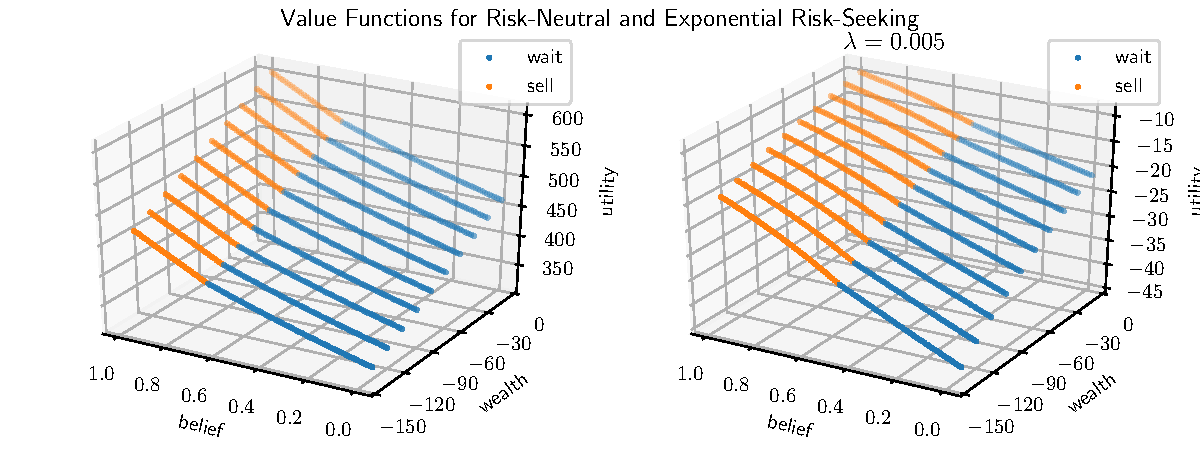
\includegraphics[width=0.9\linewidth]{img/exp_policy.pdf}\\
    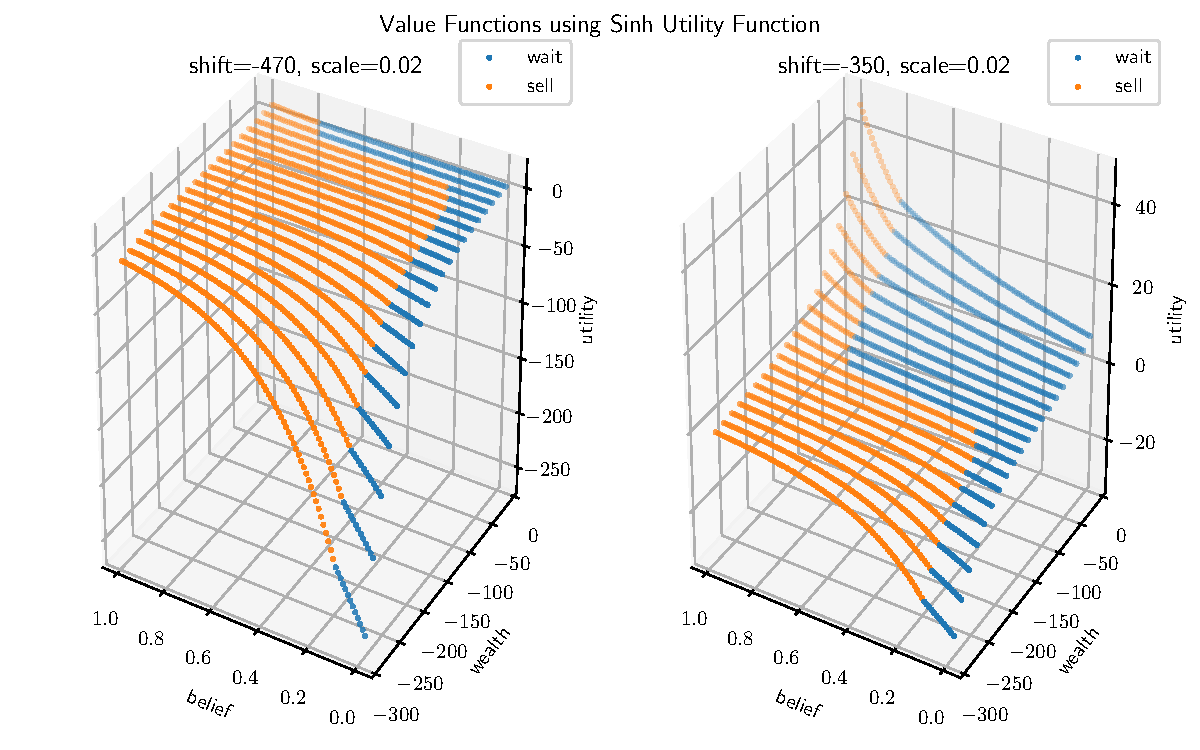
\includegraphics[width=0.9\linewidth]{img/sinh_policy.pdf}\\
    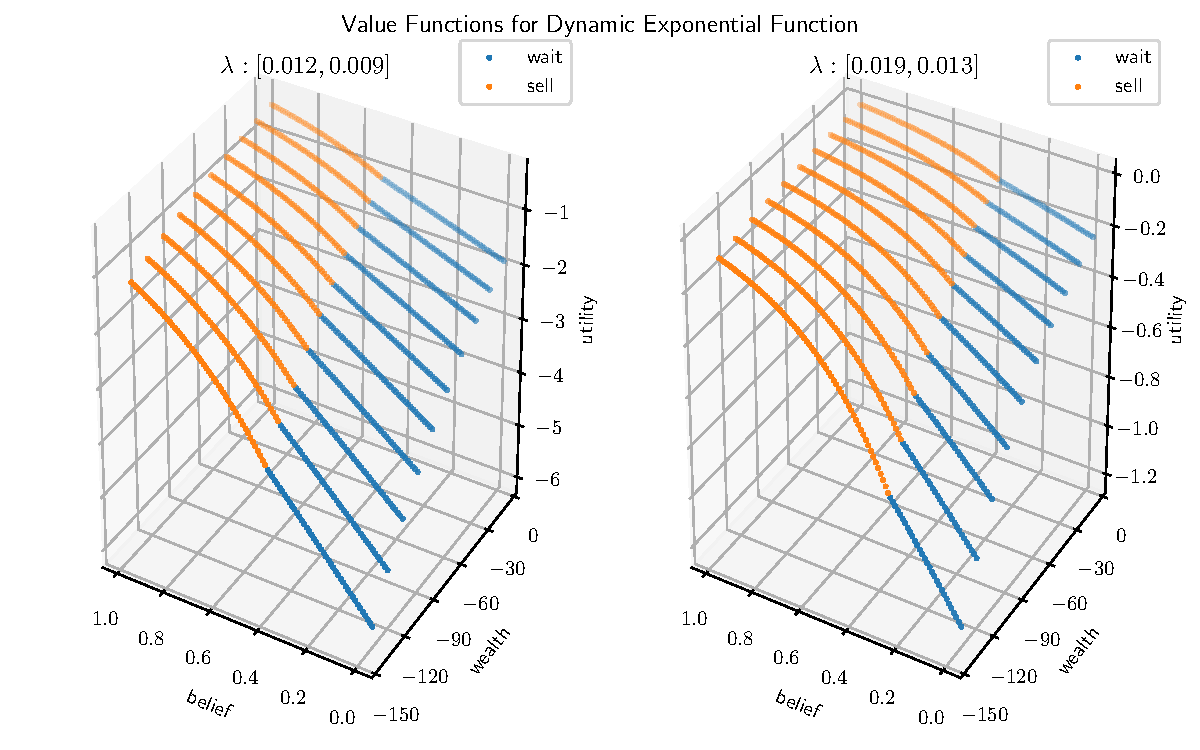
\includegraphics[width=0.9\linewidth]{img/dyn_policy.pdf}
    \caption{Value functions exhibiting different risk-behaviors; from top left: risk neutral agent (utility function is the identity function), risk-seeking agent with exponential utility function, two fixed time agents with different time thresholds, two agents with dynamic exponential utility function in the expensive expert scenario.}
\end{figure}

\textbf{The original problem:}
\begin{itemize}
\item[①] Choose Utility Function with Risk Parameter
\item[②] Perform Value Iteration
\item[③] Derive Policy
\end{itemize}

\textbf{The inverse problem:}
\begin{itemize}
\item[①] Observe Policy
\item[②] ???
\item[③] Derive utility function and risk parameters
\end{itemize}
The original problem is easy to solve, unfortunately for the inverse problem no solution is known. $\rightarrow$ Perform gridsearch and choose optimal utility function.
